\documentclass{article}
\renewcommand{\familydefault}{\sfdefault}
\usepackage{amsmath}
\usepackage{tikz}
\usetikzlibrary{positioning,arrows.meta,calc}
\pagestyle{empty}
\definecolor{enc}{RGB}{214,234,240}
\definecolor{encb}{RGB}{58,128,150}
\definecolor{cheap}{RGB}{226,239,220}
\definecolor{cheapb}{RGB}{88,140,72}
\definecolor{dec}{RGB}{252,228,214}
\definecolor{decb}{RGB}{196,110,60}
\definecolor{llm}{RGB}{233,224,244}
\definecolor{llmb}{RGB}{120,90,160}
\definecolor{store}{RGB}{222,232,250}
\newcommand{\ms}[1]{{\itshape\color{black!60}#1~ms}}
\newsavebox{\fig}
\begin{document}
\sbox{\fig}{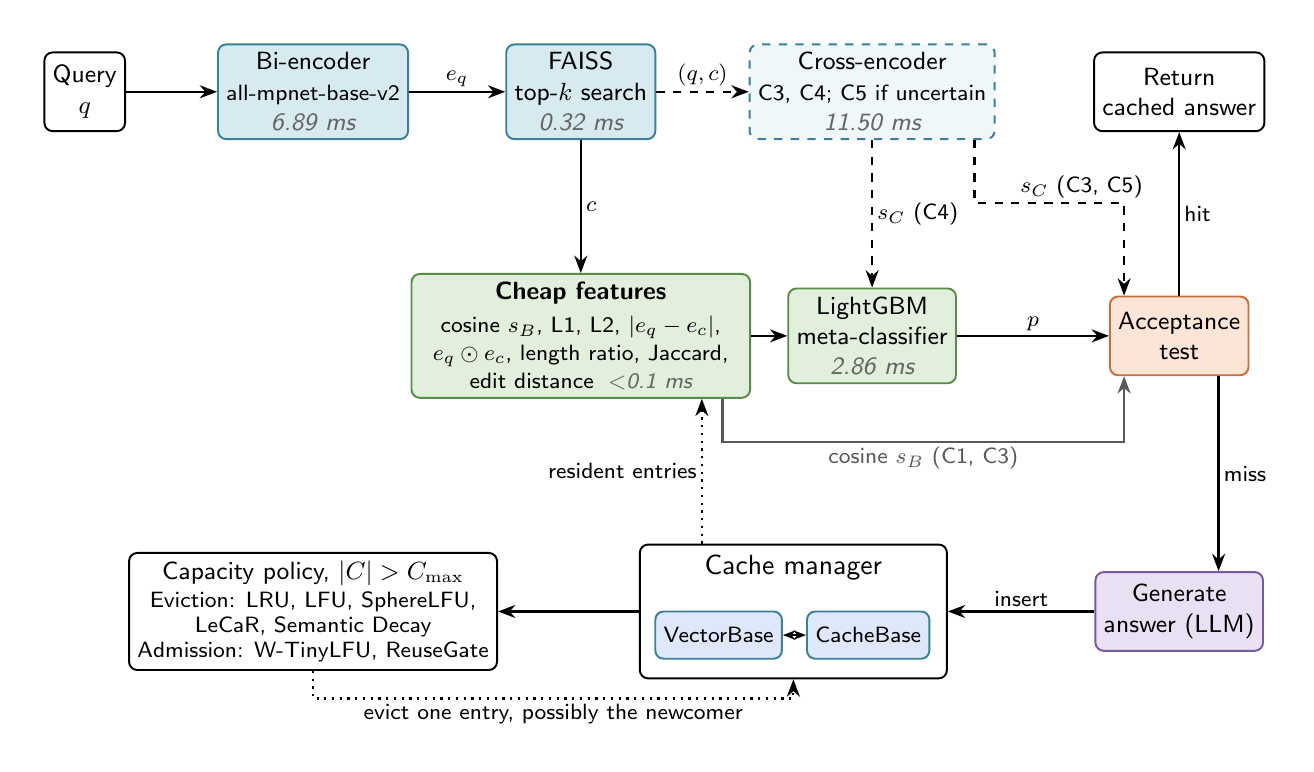
\begin{tikzpicture}[
  box/.style={draw, rounded corners=3pt, line width=0.7pt, align=center, font=\small, inner sep=3pt, minimum height=1.0cm},
  arr/.style={-{Stealth[length=2.2mm]}, line width=0.8pt},
  darr/.style={-{Stealth[length=2.2mm]}, line width=0.8pt, dashed},
  lab/.style={font=\footnotesize, inner sep=1.5pt}]

% ---- row 1: retrieval, cross-encoder, answer ----
\node[box] (q) at (0,0) {Query\\$q$};
\node[box, fill=enc, draw=encb] (bi) at (2.9,0) {Bi-encoder\\{\footnotesize all-mpnet-base-v2}\\\ms{6.89}};
\node[box, fill=enc, draw=encb] (faiss) at (6.3,0) {FAISS\\top-$k$ search\\\ms{0.32}};
\node[box, dashed, fill=enc!40, draw=encb] (ce) at (10.0,0) {Cross-encoder\\{\footnotesize C3, C4; C5 if uncertain}\\\ms{11.50}};
\node[box] (ret) at (13.9,0) {Return\\cached answer};

% ---- row 2: decision ----
\node[box, fill=cheap, draw=cheapb, minimum height=1.4cm, minimum width=4.3cm] (feat) at (6.3,-3.1)
  {\textbf{Cheap features}\\[1pt]{\footnotesize cosine $s_B$, L1, L2, $|e_q-e_c|$,}\\[-1pt]{\footnotesize $e_q\odot e_c$, length ratio, Jaccard,}\\[-1pt]{\footnotesize edit distance \;\ms{$<$0.1}}};
\node[box, fill=cheap, draw=cheapb] (lgb) at (10.0,-3.1) {LightGBM\\meta-classifier\\\ms{2.86}};
\node[box, fill=dec, draw=decb] (acc) at (13.9,-3.1) {Acceptance\\test};

\draw[arr] (q) -- (bi);
\draw[arr] (bi) -- node[lab, above]{$e_q$} (faiss);
\draw[darr] (faiss) -- node[lab, above]{$(q,c)$} (ce);
\draw[arr] (faiss) -- node[lab, right]{$c$} (feat);
\draw[arr] (feat) -- (lgb);
\draw[arr] (lgb) -- node[lab, above]{$p$} (acc);
\draw[arr] (acc) -- node[lab, right]{hit} (ret);
\draw[darr] (ce) -- node[lab, right]{$s_C$ (C4)} (lgb);
\draw[darr] ($(ce.south)+(1.3,0)$) -- ++(0,-0.8) -| node[lab, pos=0.2, above, xshift=6mm]{$s_C$ (C3, C5)} ($(acc.north)+(-0.7,0)$);
\draw[arr, black!65] ($(feat.south)+(1.8,0)$) -- ++(0,-0.55) -| node[lab, pos=0.25, below]{cosine $s_B$ (C1, C3)} ($(acc.south)+(-0.7,0)$);

% ---- row 3: miss path and capacity management ----
\node[box, fill=llm, draw=llmb] (gen) at (13.9,-6.6) {Generate\\answer (LLM)};
\draw[arr] ($(acc.south)+(0.5,0)$) -- node[lab, right]{miss} ($(gen.north)+(0.5,0)$);
\node[box, minimum width=3.9cm, minimum height=1.7cm] (cm) at (9.0,-6.6) {};
\node[anchor=north] at ($(cm.north)+(0,-0.03)$) {Cache manager};
\node[box, fill=store, draw=encb, minimum width=1.5cm, minimum height=0.6cm, font=\footnotesize] (vb) at ($(cm.center)+(-0.95,-0.3)$) {VectorBase};
\node[box, fill=store, draw=encb, minimum width=1.5cm, minimum height=0.6cm, font=\footnotesize] (cb) at ($(cm.center)+(0.95,-0.3)$) {CacheBase};
\draw[{Stealth[length=1.6mm]}-{Stealth[length=1.6mm]}, line width=0.6pt] (vb) -- (cb);
\draw[arr] (gen) -- node[lab, above]{insert} (cm);
\node[box] (ev) at (2.9,-6.6) {Capacity policy, $|C|>C_{\max}$\\[-1pt]{\footnotesize Eviction: LRU, LFU, SphereLFU,}\\[-2pt]{\footnotesize LeCaR, Semantic Decay}\\[-2pt]{\footnotesize Admission: W-TinyLFU, ReuseGate}};
\draw[arr] (cm) -- (ev);
\coordinate (r0) at ($(cm.north west)+(0.8,0)$);
\draw[arr, dotted] (r0) -- node[lab, left, pos=0.5]{resident entries} (r0 |- feat.south);
\draw[arr, dotted] (ev.south) -- ++(0,-0.35) -| node[lab, pos=0.25, below]{evict one entry, possibly the newcomer} (cm.south);

\path ([shift={(-2mm,-2mm)}]current bounding box.south west) rectangle ([shift={(2mm,2mm)}]current bounding box.north east);
\end{tikzpicture}}%
\pdfpagewidth=\wd\fig \pdfpageheight=\dimexpr\ht\fig+\dp\fig\relax
\hoffset=-1in \voffset=-1in \oddsidemargin=0pt \topmargin=0pt \headheight=0pt \headsep=0pt
\textwidth=\wd\fig \parindent=0pt
\noindent\usebox{\fig}
\end{document}
